\subsection{Question 1}
\subsubsection{Question 1.1}

Soit $f=(f_{d_0}\ f_{p_0}\ f_{p_1}\ f_{f_0}\ f_{c_0}\ f_{c'_0})$ le vecteur générique de P-semi-flots.\\
Tina nous donne le p-semi-flot suivant pour le premier schéma :\\
\begin{center}
  $f= (1\ 1\ 1\ 1\ 0\ 0)$

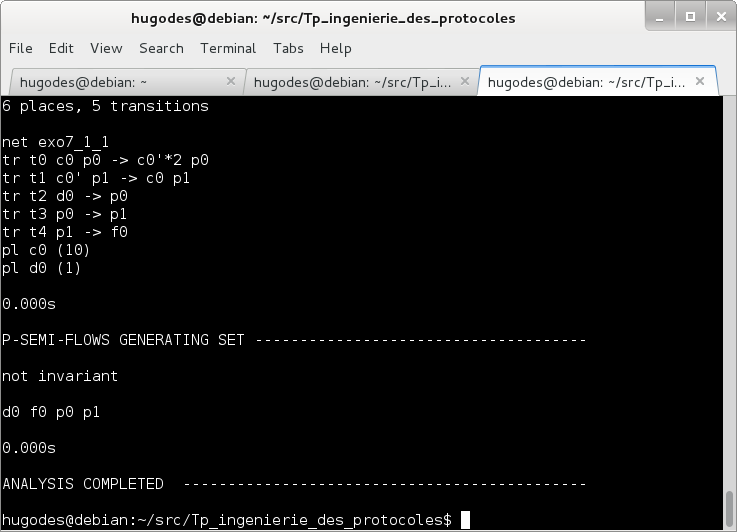
\includegraphics[width=0.7\textwidth]{exo7/tina_7_1.png}\\

\end{center}

On va utiliser l'algorithme de Farkas pour calculer les P-semi flots du premier schéma.

\begin{center}

{\Huge C}\qquad =\qquad $\bordermatrix{
&t_1&t_2&t_3&t_4&t_5\cr
d0&-1&0&0&0&0\cr
p0&1&-1&0&0&0\cr
p1&0&1&-1&0&0\cr
f0&0&0&1&0&0\cr
c0&0&0&0&-1&1\cr
c'0&0&0&0&2&-1\cr
}$

{\Huge $\downarrow$}

$\bordermatrix{
&t_2&t_3&t_4&t_5\cr
d0+p0&-1&0&0&0\cr
p1&1&-1&0&0\cr
f0&0&1&0&0\cr
c0&0&0&-1&1\cr
c'0&0&0&2&-1\cr
}$

{\Huge $\downarrow$}

$\bordermatrix{
&t_3&t_4&t_5\cr
d0+p0+p1&-1&0&0\cr
f0&1&0&0\cr
c0&0&-1&1\cr
c'0&0&2&-1\cr
}$

{\Huge $\downarrow$}

$\bordermatrix{
&t_4&t_5\cr
d0+p0+p1+f0&0&0\cr
c0&-1&1\cr
c'0&2&-1\cr
}$


\vspace{1cm}

On trouve donc un P-semi flot :\\
$f = (1\ 1\ 1\ 1\ 0\ 0)$

On obtient donc le même résultat que TINA.

\end{center}


\subsubsection{Question 1.2}

Soit $f=(f_{c_i}\ f_{c'_i}\ f_{c_{i-1}}\ f_{d_i}\ f_{d_{i-1}}\ f_{f_{i-1}}\ f_{f_i}\ f_{p_1})$ le vecteur générique de P-semi-flots.\\

Tina nous donne le p-flot suivant pour le second schéma :\\

\begin{center}

$f_1 = (0\ 1\ 1\ 0\ 0\ 0\ 0\ 0)$\\
$f_2 = (0\ 0\ 1\ 1\ 1\ 0\ 0\ 1)$\\

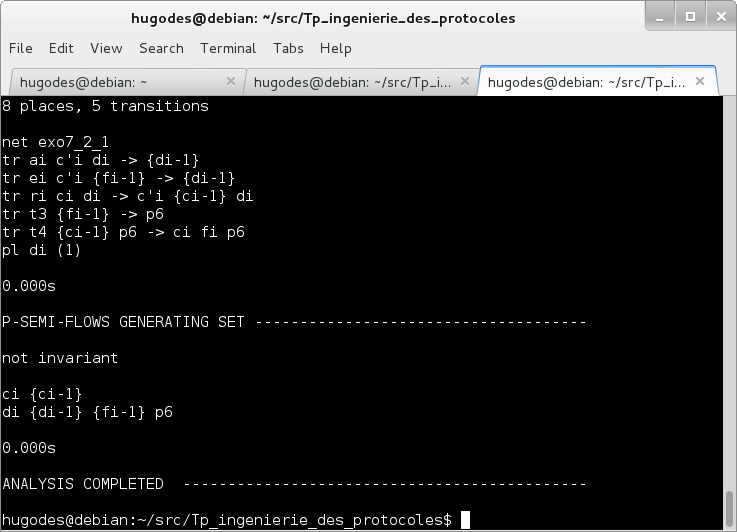
\includegraphics[width=0.7\textwidth]{exo7/tina_7_2.png}\\

\end{center}

On va utiliser l'algorithme de Farkas pour calculer les P-semi flots du second schéma.

\begin{center}


{\Huge C}\qquad =\qquad $\bordermatrix{
&ai&ei&ri&t1&t2\cr
ci&0&0&-1&0&1\cr
c'i&-1&-1&1&0&0\cr
ci-1&0&0&1&0&-1\cr
di&-1&0&0&0&0\cr
di-1&1&1&0&0&0\cr
fi-1&0&-1&0&-1&0\cr
fi&0&0&0&0&1\cr
p1&0&0&0&1&0\cr
}$

{\Huge $\downarrow$}

$\bordermatrix{
&ei&ri&t1&t2\cr
ci&0&-1&0&1\cr
c'i+di-1&0&1&0&0\cr
ci-1&0&1&0&-1\cr
di+di-1&1&0&0&0\cr
fi-1&-1&0&-1&0\cr
fi&0&0&0&1\cr
p1&0&0&1&0\cr
}$

{\Huge $\downarrow$}

$\bordermatrix{
&ri&t1&t2\cr
ci&-1&0&1\cr
c'i+di-1&1&0&0\cr
ci-1&1&0&-1\cr
di+di-1+fi-1&0&-1&0\cr
fi&0&0&1\cr
p1&0&1&0\cr
}$

{\Huge $\downarrow$}

$\bordermatrix{
&t1&t2\cr
c'i+di-1+ci&0&1\cr
ci-1+ci&0&0\cr
di+di-1+fi-1&-1&0\cr
fi&0&1\cr
p1&1&0\cr
}$

{\Huge $\downarrow$}

$\bordermatrix{
&t2\cr
c'i+di-1+ci&1\cr
di+di-1+fi-1+p1&0\cr
fi&1\cr
}$

\vspace{1cm}

On trouve donc 2 P-semi flots :\\
$f_1 = (0\ 1\ 1\ 0\ 0\ 0\ 0\ 0)$\\
$f_2 = (0\ 0\ 1\ 1\ 1\ 0\ 0\ 1)$\\

\end{center}

On obtient donc le même résultat que TINA.


\subsection{Question 2}
\subsubsection{Question 2.1}
Pour le premier schéma la séquence maximale est:\\
t1 -> n*t4 -> t2 -> 2n*t5 -> t3

\subsubsection{Question 2.2}
Pour le second schéma la séquence maximale est:\\
ri -> ai -> ri-1 -> ai-1 -> ... -> ri-n -> ai-n


\subsection{Question 3}
\subsubsection{Question 3.1}

Nous pouvons construire le graphe de marquage suivant pour la première figure:

\begin{figure}[H]
  \centering
  \begin{tikzpicture}
    % Liste des Marquage
    \node (M0) at (-6,6) {$(1\ 0\ 0\ n\ 0\ 0)$};
    \node (M1) at (-6,4) {$(0\ 1\ 0\ n\ 0\ 0)$};
    \node (M2) at (0,2) {$(0\ 0\ 1\ n\ 0\ 0)$};
    \node (M3) at (-6,2) {$(0\ 1\ 0\ n-i\ 2*i\ 0)$};
    \node (M4) at (-6,0) {$(0\ 0\ 1\ n-i\ 2*i\ 0)$};
    \node (M5) at (0,-2) {$(0\ 0\ 0\ n-i\ 2*i\ 1)$};
    \node (M6) at (-6,-2) {$(0\ 0\ 1\ n-i+j\ 2*i-j\ 0)$};
    \node (M7) at (-6,-4) {$(0\ 0\ 0\ n-i+j\ 2*i-j\ 1)$};

     % Liste des arcs
    \draw[->,>=latex] (M0) -- (M1) node[midway, right]{$t_1$};
    \draw[->,>=latex] (M1) -- (M2) node[midway, right]{$t_2$};
    \draw[->,>=latex] (M1) -- (M3) node[midway, right]{$t_4$};
    \draw[->,>=latex] (M3) -- (M4) node[midway, right]{$t_2$};
    \draw[->,>=latex] (M4) -- (M5) node[midway, right]{$t_3$};
    \draw[->,>=latex] (M4) -- (M6) node[midway, right]{$t_5$};
    \draw[->,>=latex] (M6) -- (M7) node[midway, right]{$t_3$};

  \end{tikzpicture}
  \caption{Graphe des marquages accessibles} \label{fig:M10}
\end{figure}

$\forall S_i, \forall S_j \in A M_{S_j} = M_{S_i} \rightarrow S_i = S_j$

Donc le graphe de couverture est égal à l'arbre.

\subsubsection{Question 3.2}

Nous pouvons construire le graphe de marquage suivant pour la deuxième figure:

\begin{figure}[H]
  \centering
  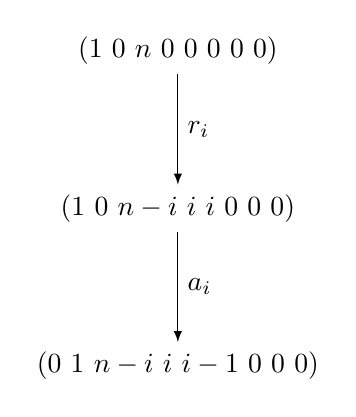
\begin{tikzpicture}
    % Liste des Marquage
    \node (M0) at (-6,6) {$(1\ 0\ n\ 0\ 0\ 0\ 0\ 0)$};
    \node (M1) at (-6,4) {$(1\ 0\ n-i\ i\ i\ 0\ 0\ 0)$};
    \node (M2) at (-6,2) {$(0\ 1\ n-i\ i\ i-1\ 0\ 0\ 0)$};


     % Liste des arcs
    \draw[->,>=latex] (M0) -- (M1) node[midway, right]{$r_i$};
    \draw[->,>=latex] (M1) -- (M2) node[midway, right]{$a_i$};


  \end{tikzpicture}
  \caption{Graphe des marquages accessibles} \label{fig:M10}
\end{figure}

$\forall S_i, \forall S_j \in A M_{S_j} = M_{S_i} \rightarrow S_i = S_j$

Donc le graphe de couverture est égal à l'arbre.

\subsection{Question 4}

En faisaint varrier les nombre de jetons dans les places on remarque que TINA ne gère pas des nombres de jetons variable (j'usqu'a l'inifni). Cela résulte dans le fait que l'on se retrouve avec des graphes / arbres de marquage qui explosent.
